\documentclass{article}
\usepackage[utf8]{inputenc}
\usepackage{amsmath}
\usepackage{graphicx}

\title{Eksamensdisposition - Divide and Conquer}

\author{André Oskar Andersen (wpr684)}

\date{\today}

\begin{document}

\maketitle

\begin{itemize}
    \item Paradigmet:
    \begin{itemize}
        \item Hvad menes der ved \textit{Divide}?
        \item Hvad menes der ved \textit{Conquer}?
        \item Hvad menes der ved \textit{Combine}?
    \end{itemize}
    \item Eksempel på \textit{divide-and-conquer}; håndkørsel af merge sort på $\{5, 2, 4, 7\}$
    \item \textit{Recurrences}:
    \begin{itemize}
        \item Hvad er en \textit{recurrence}?
        \item Hvordan løses en \textit{recurrence}?
        \begin{itemize}
            \item \textit{Recursion-tree method}
            \item \textit{Substitution method}
            \item \textit{Master method} (kort)
        \end{itemize}
    \end{itemize}
    \item \textit{Comparison sort}:
    \begin{itemize}
        \item Hvad er en \textit{comparison sort}?
        \item Bevis for \textit{lower bound} for \textit{comparison sort}
    \end{itemize}
\end{itemize}

\newpage

\section*{Forberedelsesnoter}
\subsection*{Paradigmet}
\subsubsection*{Hvad menes der ved \textit{Divide}?}
\begin{itemize}
    \item \textit{Divide}: Del problemet i flere delproblemer der er mindre instanser af det originale problem
\end{itemize}
\subsubsection*{Hvad menes der ved \textit{Conquer}?}
\begin{itemize}
    \item \textit{Conquer}: Løs delproblemerne rekursivt. Er problemerne tilpas små, løses de bare "direkte"
\end{itemize}
\subsubsection*{Hvad menes der ved \textit{Combine}?}
\begin{itemize}
    \item \textit{Combine}: Kombiner delproblemernes løsning til én samlet løsning for det originale problem.
\end{itemize}
\subsection*{Håndkørsel af merge sort}
\begin{center}
    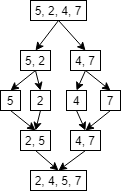
\includegraphics[height = 5 cm]{../entities/merge_sort_example.png}
\end{center}
\begin{itemize}
    \item For at gøre det nemmere, viser jeg et eksempel, hvor array'et har en længde som er en eksponent af 2 - algoritmen virker dog stadig hvis dette ikke gælder.
    \item Algoritmen starter ud ved at dele array'et op, rekursivt, indtil den har \textit{n} arrays, hver med størrelsen $1$.
    \item Når algoritmen har \textit{n} arrays af hver størrelsen $1$, "bottom'er" algoritmen ud og begynder at kombinere array'ene
    \item Algoritmen kombinerer array'ene, ved at have en pointer til det mindste element i de to arrays (det første element, idet array'ene er sorteret). Herefter "trækker den" det mindste element, og rykker pointeren frem i det array, der lige er trukket fra. Dette gøres, indtil ét af arrays'ne er tomme. Herefter trækker den alle elementer ned fra den modsatte array. Dette sker rekursivt, indtil algoritmen ender ud med kun ét array.
\end{itemize}

\subsection*{\textit{Recurrences}}
\subsubsection*{Hvad er en recurrence?}
\begin{itemize}
    \item En \textit{recurrence} bruges ofte til at beskrive en algoritmes køretid, når den gør brug af rekursion. Dette ses eksempelvis på \textit{merge sort}, der har rekursionsligningen
    \[
        T(n) =
        \begin{cases}
            c & \text{if $n = 1$} \\
            2T(n/2) + c & \text{if $n > 1$}
        \end{cases} 
    \]
    hvor \textit{c} repræsenterer tiden det tager at løse delproblemer med størrelsen $1$ og tiden det tager at dele og kominere arrays. Dette kan dog omskrives til
    $$T(n) = 2T(n/2) + cn$$
    Selvom $T(1)$ vil resultere i noget andet, så vil løsningen ikke ændres med mere end en konstant og derfor vil ikke have en effekt på køretiden. \\
    Floor og ceiling bliver og ignoreret, idet vi tager udgangspunkt i at kalde mergesort på et array af en ekponent af 2. \\
    Vi får hertil denne rekursionsligning, idet vi får 2 delarrays, der hver er af den halvestørrelse, samt får $cn$, da vi også skal bruge tid på at dele og samle array'ene.
\end{itemize}
\subsubsection*{Hvordan løses en recurrence?}
\begin{center}
    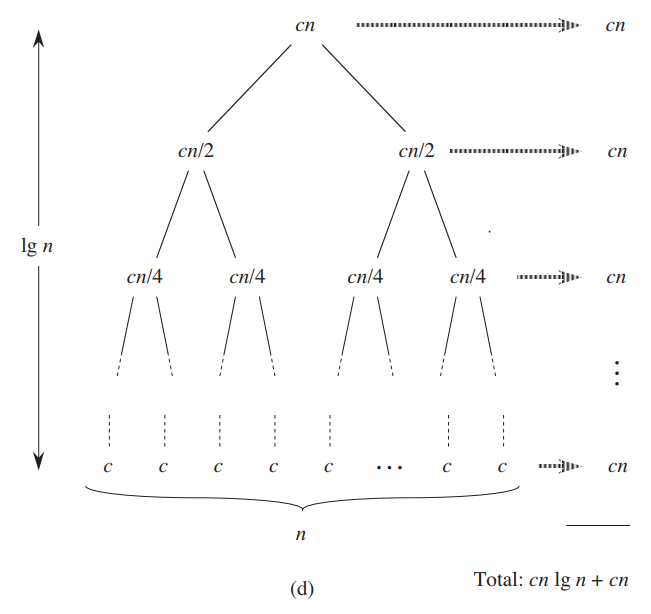
\includegraphics[width = 10 cm]{../entities/merge_sort_recursion_tree.png}
\end{center}
\textbf{Recursion-tree method}
\begin{itemize}
    \item Et rekursionstræ bruges til at komme med et godt gæt af køretiden, som så kan bevises ved hjælp af substitutionsmetoden. Er man meget præcis, kan rekursionstræet dog også bruges til at bevise rekursionsligningen.
    \item Hver knud repræsenterer omkostningerne af den ikke-rekursive del af kaldet et enkelt delproblem.
    \item I merge sort's rekursionstræ ses det, at hvert niveau's omkostninger er $cn$, samt der er $\lg n$ af disse. Derfor gætter vi på, at køretiden af merge sort er $O(n \lg n)$
\end{itemize}
\textbf{Substitution method}
\begin{itemize}
    \item Substitutionsmetoden fungerer ved, at
    \begin{enumerate}
        \item Komme med et gæt på løsningen (eksempelvis ved hjælp af et rekursionstræ), på køretiden
        \item Bevis løsningen ved hjælp af induktion
    \end{enumerate}
    \item Løsning af \textit{recurrence} $T(n) = 2T(\left \lfloor{n/2}\right \rfloor) + n$:
    \begin{enumerate}
        \item Vi skal bevise $T(n) \leq cn \lg n$
        \item Vi antager, at $T(1) = 1$
        \item Lader vi $n = 1$, findes der ikke en løsning for $T(n) \leq cn \lg n$, da $cn \lg n = 0$. Istedet beviser vi det for $n \geq 2$ og lader $n_0 = 2$.
        \item Da $T(1) \leq c \cdot 1 \lg 1$ ikke gælder, har vi brug for 2 base cases; $n = 2$ og $n = 3$ \\
        \item \textbf{Base case:} Fra ligningen kan vi se, at $T(2) = 4$ og $T(3) = 5$. Lader vi $c = 2$ har vi $T(n) \leq cn \lg n$ for $n = 2, 3$.
        \item \textbf{Induktionsskridt}:
        $$T(n) = 2T(\left \lfloor{n/2} \right \rfloor) + n$$
        $$\leq 2(c \left \lfloor{n/2} \right \rfloor \lg(\left \lfloor{n/2} \right \rfloor)) + n$$
        $$\leq cn \lg(n/2) + n$$
        $$= cn \lg n - cn \lg 2 + n$$
        $$= cn \lg n - cn + n$$
        $$\leq cn \lg n$$
    \end{enumerate}
\end{itemize}
\textbf{Master method}
\begin{itemize}
    \item \textit{Master method}'en kan bruges til at løse rekursionsligninger på formen
    $$T(n) = aT(n/b) + f(n)$$
    hvor $a \geq 1$ og $b > 1$ er konstanter og $f(n)$ er en asymptotisk positiv funktion.
\end{itemize}
\subsection*{\textit{Comparison sort}}
\subsubsection*{Hvad er en \textit{comparison sort}}
\begin{itemize}
    \item I en \textit{comparison sort} gøres der kun brug af sammenligninger imellem elementer til at sortere et array.
\end{itemize}
\subsubsection*{Bevis for \textit{lower bound} for \textit{comparison sort}}
\begin{itemize}
    \item Vi starter med at antage, at alle elementer er forskellige. Herved er operationer som $a_i = a_j$ ubrugelige. Hertil giver alle andre operationer den samme mængde information. Derfor antager vi, at alle sammenligninger er på formen $a_i < a_j$
    \item Vi kan se på en \textit{comparison sort}, som et \textit{decision tree}, hvor hvert blad er en permutation af input array'et.
    \item Udførelsen af sorteringsalgoritmen kan herved ses, som at gå ned igennem træet, fra roden til et blad. Hver indvendig knude indikerer en sammenligning; går man herefter til venstre gjaldt det, at $a_i < a_j$ - går man modsat til højre gjaldt det, at $a_i \leq a_j$.
    \item Højden af træet beskriver værste tilfælde af sammenligninger der udføres. Derved, et lower-bound på højden er derfor også et lower bound på køretiden af hvilken som helst \textit{comparison sort}.
    \item Vi lader antallet af blade være \textit{b} og højden \textit{h}. Er træet perfekt balanceret kan vi presse $2^h$ blade ind i træet. Vi ved også, at alle permutationer forekommer i bladene, derfor må $b \geq n!$, da der ellers ikke ville være plads til alle permutationer i bladene. Defor får vi
    $$2^h \geq b \geq n!$$
    Tager vi $\lg$, får vi
    $$h \geq \lg(n!) = \Omega(n \lg n)$$
    \item Siden $O(n \lg n)$ er køretiden for merge sort, hvilket matcher lower bound for comparison sort worst-case; $\Omega(n \lg n)$, er mege sort asymptotisk optimal.
\end{itemize}
\end{document}